\documentclass{homework}
% \usepackage{lua-visual-debug}
\usepackage{graphicx}
\usepackage{float}
\usepackage{minted}

\title{Practice \#1}
\subject{CS341 Introduction to Computer Networks}
\studentid{20170058}
\name{Keonwoo Kim}
\date{\today}

\AtBeginEnvironment{minted}{\singlespacing\fontsize{9}{12}\selectfont}
\newminted{latex}{breaklines=true,breaksymbolleft={}}
\usemintedstyle{manni}
\setminted{bgcolor=white!95!black}
\setmintedinline{fontsize=\small}

\begin{document}
\maketitle

\begin{figure}[H]
  \centering
  \vspace*{-2em}
  \hspace*{-0.2\textwidth}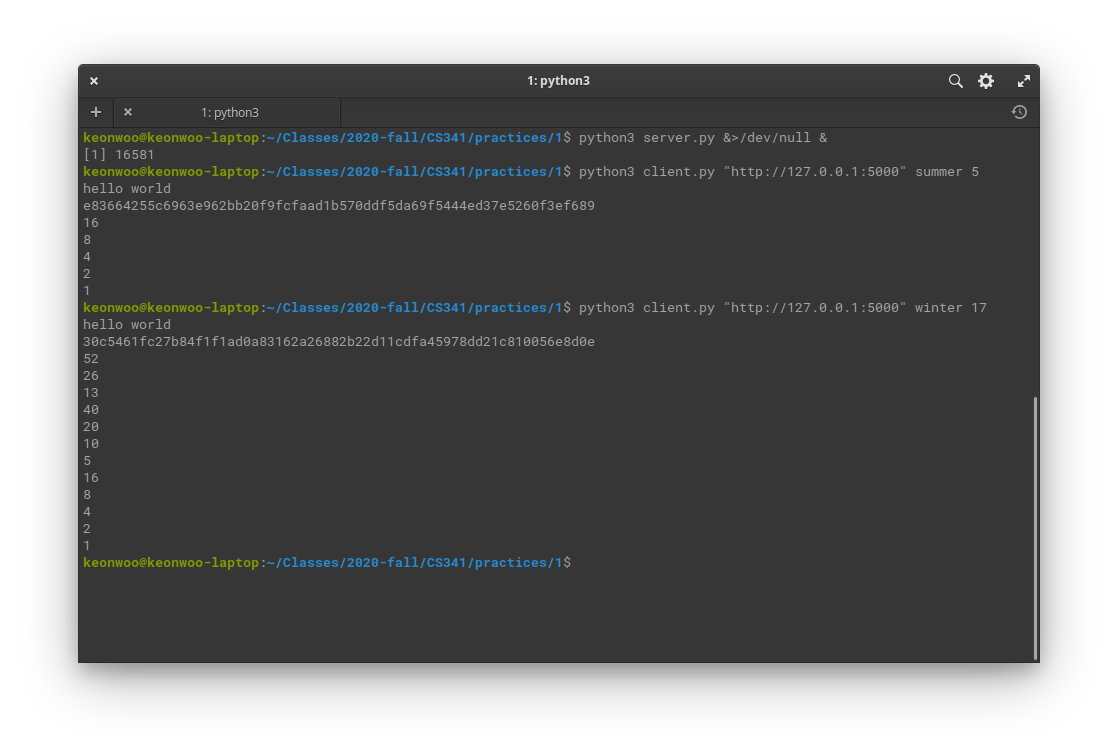
\includegraphics[width=1.4\textwidth]{screenshot}
  \vspace*{-4em}
  \caption{The screenshot of working server and client.}
\end{figure}
\vspace*{2em}

The following is the code of the file \mintinline{text}{server.py}, with detailed and descriptive comments added.

\begin{minted}[fontsize=\footnotesize]{python}
# server.py

from flask import Flask, render_template, request
import json
import hashlib

# create a Flask app
app = Flask(__name__)

@app.route('/hello_world', methods=['GET'])
def route_hello_world():
    # send the hello world message to the client
    return json.dumps({'message': 'hello world'})

@app.route('/hash', methods=['GET'])
def route_hash():
    # get the name from the GET url parameters
    name = request.args.get('name')

    # hash the name parameter
    hash = hash_sha256(name)

    # send it to the client
    return json.dumps({'result': hash})

@app.route('/collatz', methods=['POST'])
def route_collatz():
    # get the name and the hash value from the POST data
    name = request.form.get('name')
    hash_in_request = request.form.get('hash')

    # hash the name parameter and compare with the requested one
    hash = hash_sha256(name)
    if hash != hash_in_request:
        return json.dumps({'error': 'HASH NOT MATCHED'})

    # get the number from the POST data
    number = request.form.get('number')
    # try to convert it to an integer
    try:
        # if it is an integer,
        # send the result of the collatz function to the client
        return json.dumps({'result': collatz(int(number))})
    except ValueError:
        # elsewise, show the error to the client
        return json.dumps({'error': 'NUMBER NOT INTEGER'})

# hash function
def hash_sha256(text):
    return hashlib.sha256(text.encode()).hexdigest()

# collatz function
def collatz(number):
    if number % 2 == 0:
        return int(number / 2)
    return 3 * number + 1

# run the Flask app
if __name__ == '__main__':
    app.run()
\end{minted}

The following is the code of the file \mintinline{text}{client.py}, with detailed and descriptive comments added.

\begin{minted}[fontsize=\footnotesize]{python}
# client.py

import sys
import requests

# get url, name, and number parameters from the terminal
url = sys.argv[1]
name = sys.argv[2]
number = int(sys.argv[3])

# send a GET request to /hello_world and shows the message the client got
hello_world_response = requests.get(url + '/hello_world')
print(hello_world_response.json().get('message'))

# send a GET request to /hash with the name parameter
# and shows the result the client got
hash_response = requests.get(url + '/hash', params={'name': name})
hash = hash_response.json().get('result')
print(hash)

# while the client got 1
while number != 1:
    # send a POST request to /collatz
    # with the POST data including `name`, `hash` and `number`
    collatz_response = requests.post(
        url + '/collatz', data={'name': name, 'hash': hash, 'number': number})
    
    # convert the response data into a python dict
    collatz_response_dict = collatz_response.json()

    # if the response has the `error' field, raise an Exception
    if 'error' in collatz_response_dict:
        raise Exception('ERROR: ' + collatz_response_dict.get('error'))

    # save the collatz result into `number`, print it,
    # and repeat the process
    number = collatz_response_dict.get('result')
    print(number)

\end{minted}

\end{document}